\FloatBarrier
\subsection{Site specific noise}
As was mentioned in the reference design section, it is of great importance to determine if sites contain already existing infrastructure, what the depth of the site is, and what the geologic and seismologic stability is at a given location. This last point is because site specific noise sources, like for instance seismic noise, will most likely influence the final sensitivity of the ET observatory. In order to prevent that the detector sensitivity is affected by seismically induced vibrations, current gravitational wave detectors employ seismic isolation system. Details about the proposed seismic isolation strategies for ET are explained in Chapter\,4. For illustrative purposes, figure \ref{SuspensionArtistic} shows an artist cut-away impression of the 17\,m high suspension systems, proposed for the ET test masses. 
%\begin{figure}[h!]
%	\begin{center}
%		 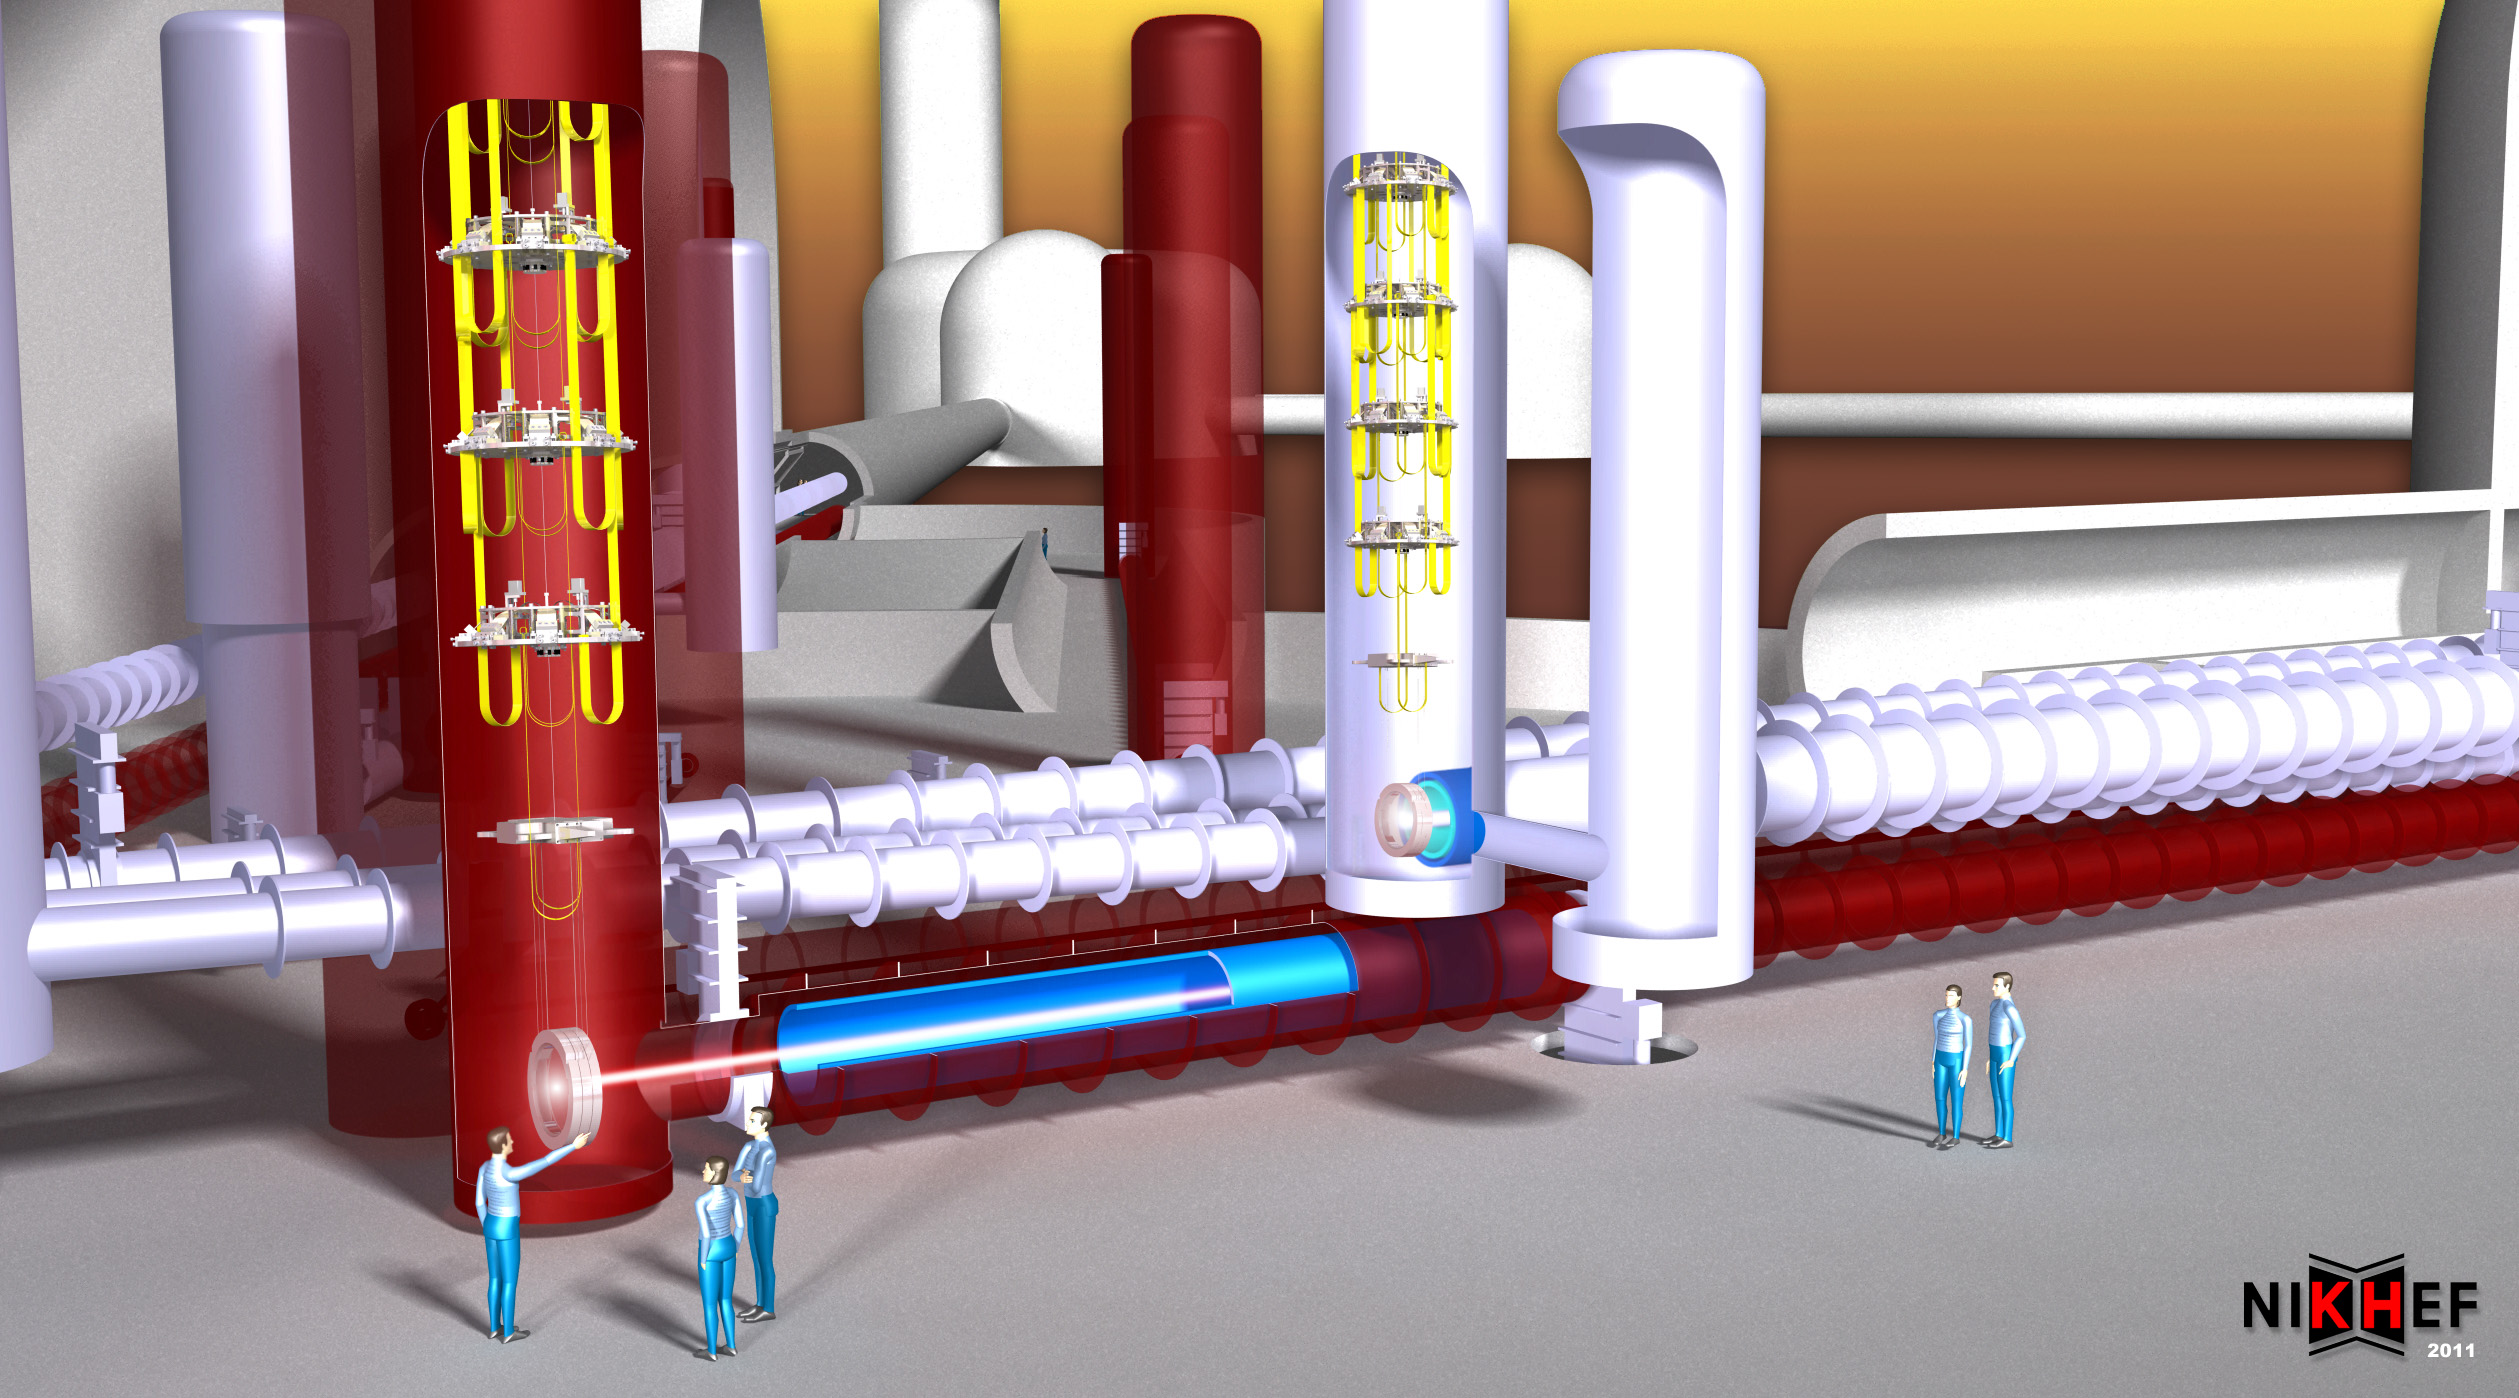
\includegraphics[width=17cm]{./Sec_SiteInfra/Figures/SuspensionArtistic2.jpg}
%			\caption{Artistic cut-away impression of the ET suspension system. Such suspension chains isolate the test-masses at the bottom from seismic disturbances. For ET, seismic isolation alone will not suffice and sites with low seismic background need to be identified.}		
%			\label{SuspensionArtistic}
%	\end{center}
%\end{figure}

%The isolation requirements for ET scale with the local seismic activity. Therefore, it is prudent to identify the areas within Europe that comply with long term stability requirements for ET and study the diurnal and seasonal variations of local seismologic, geologic, and hydrologic conditions. Section \ref{SeismicNoise} provides a background on seismic noise and its origin, for the preliminary site investigation in section \ref{SiteInvestigation}.

The seismic isolation requirements for ET scale with the local seismic activity at a given site. Thus, when scaling the seismic isolation requirements from current detectors to those for ET, it becomes clear that sites with a low seismic noise background are required to fulfil the seismic isolation target. Following in the footsteps of LCGT, site studies were therefore aimed at underground environments in Europe. The most significant results of this study are presented in \ref{SiteInvestigation}, showing the variation in local seismic activity in a variety geologies like hard rock (Frejus, Canfranc, Gran Sasso, Sardinia and Hungary in Europe, Homestake in the USA, and Kamioka in Japan), salt (Slanic Salt Mine in Romenia, and Realmonte in Sicily), and in Boom clay (the HADES facility for storage of nuclear waste in Mol, Belgium).  

%Finally, section \ref{NewtonianNoise} provides the background on a secondary site specific noise source that originates from the local seismic activity, called gravity gradient noise. Gravity gradient noise arrises from the Newtonian coupling between the soil and the interferometer test mass. The local seismic background can be regarded as a stochastic field which causes time varying density perturbations in the soil. These density variations are the cause of a direct perturbation in the local gravity field, which of the same order (or bigger) than the gravitational wave induced signal.  

\FloatBarrier
\subsubsection{Seismic noise}
\label{SeismicNoise}
Noise studies \cite{Bard2003, Gutenberg1958, Asten1984, Peck2008} often categorise seismic noise sources according to frequency. For Einstein Telescope, critical frequency regions are in the range of 0.1 - 10\,Hz, where the seismic noise is variable mainly due to microseismic and human activity. Noise at frequencies below 1\,Hz is termed `microseismic' and its sources are dominantly natural ($i.e.$ non cultural and non-local), depending on oceanic and large-scale meteorological conditions ($e.g.$ monsoons and cyclones). Around 1\,Hz wind effects and local meteorological conditions show up, while for frequencies above 1\,Hz additional sources (besides natural) are related mainly due to human activity. Such noise is termed `cultural noise' or `anthropogenic noise'. It should be noted that the 1 Hz division is not absolute.
 \begin{figure}[h!]
	\begin{center}
		 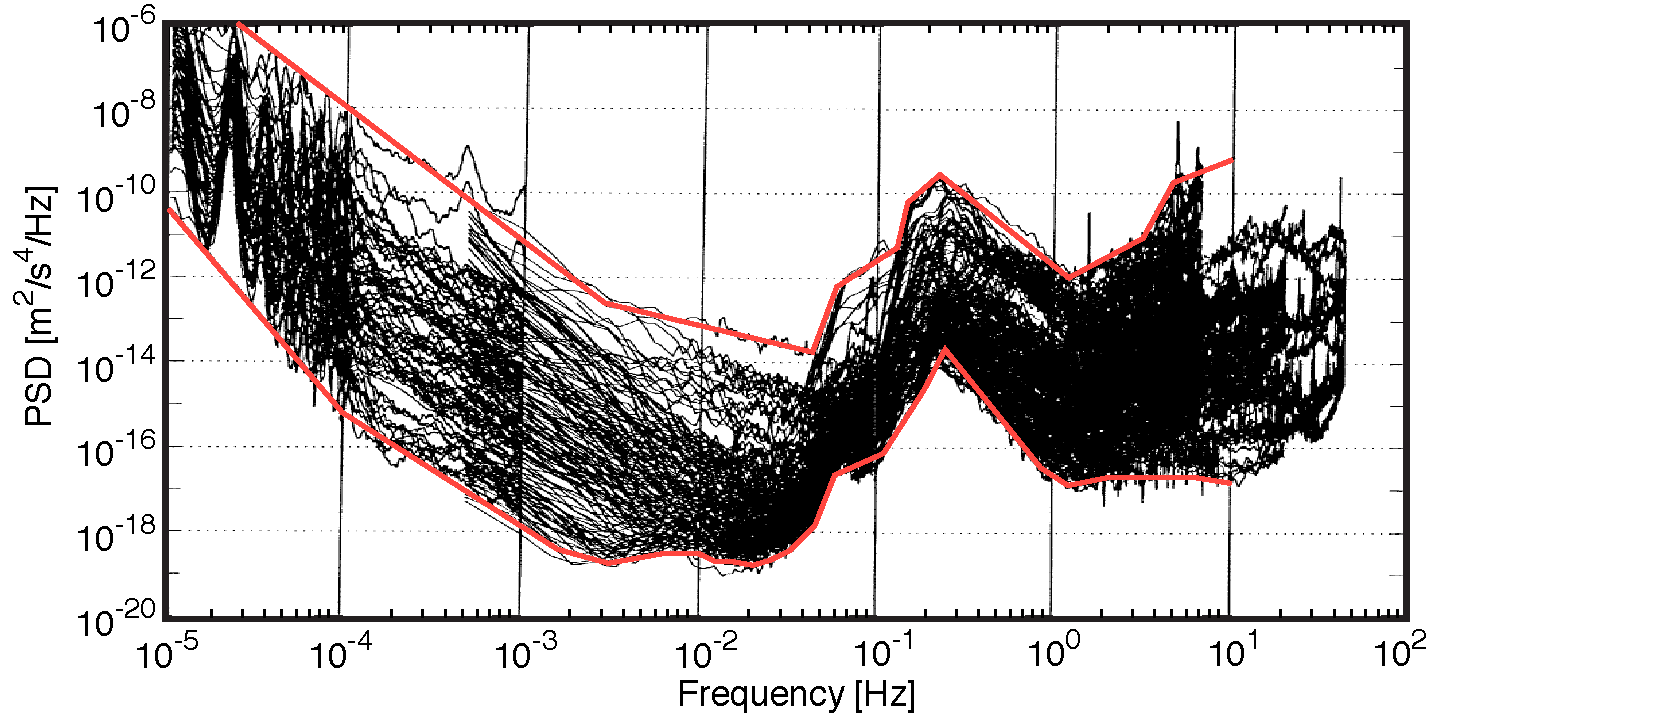
\includegraphics[width=17cm]{./Sec_SiteInfra/Figures/peterson2.pdf}
			\caption{Overlay of network station spectra used in Peterson's background noise study \cite{Peterson1993} together with straight-line segments fitted to the high-noise and low-noise envelopes of the overlay.}		
			\label{fig3.1}
	\end{center}
\end{figure}

Throughout this section seismic measurements are presented as acceleration power spectral density (PSD)\footnote{In the literature various representations are used, such as the root power spectral density (RPSD), acceleration, velocity and displacement spectral densities.} versus Fourier frequency, where PSD values have units of squared acceleration $({\rm m/s}^2)^2/{\rm Hz}$. The largest PSD values are seen at low frequencies. Here, the surface of the Earth experiences large external forces due to the gravitational attractions of the Moon and Sun. At very low frequencies this causes the surface of the Earth to rise and fall with amplitudes of about 0.5\,m with respect to the center of the Earth. This tidal motion can be seen in Fig. \ref{fig3.1} at a frequency of $2.3 \times 10^{-5}$\,Hz. Since the motion occurs at very low frequency the interferometer test masses will move {\sl coherently} and differential test mass motion presents no problem. Large PSD values are observed at frequency clustered around $5.5 \times 10^{-2}$\,Hz and 0.2\,Hz which correspond to microseisms. Note that a large dynamic range of more than eight orders of magnitude is needed to accommodate signals between 0.01\,Hz and 1\,Hz.

Peterson \cite{Peterson1993} catalogued acceleration noise power spectral density plots for frequencies up to 50\,Hz from 75 seismic stations distributed worldwide. Several years of data were collected (about 12,000 spectra in total). From the upper and lower bound of the combined data of both surface and borehole sensors (100 - 340\,m depth) Peterson derived, what is now known as, the new high/low noise model (NHNM/NLNM), which replaced his earlier low noise model \cite{Peterson1980}. The data including the upper and lower bound fit are shown in Fig. \ref{fig3.1}. 

As can be seen from Fig \ref{fig3.1}, microseismic ground motion is a prominent feature for frequencies around 0.07\,Hz and 0.17\,Hz. The small lower-frequency peak (periods of 10 - 16\,s) correlates with the frequency of coastal waves, where the ocean wave energy is converted into seismic energy through either vertical pressure variations or from the surf crashing onto the shore. The larger peak, at about twice the frequency (periods of 4 - 8\,s), originates from standing ocean waves that couple to the continental shelf. The standing waves are generated by superposition of ocean waves of equal period traveling in opposite directions and have recently been confirmed by satellite observations. Corresponding PSD values change up to 30 dB depending on the storm intensity, while the two frequencies shift upward as storms age.
\begin{figure}[t!]
	\begin{center}
		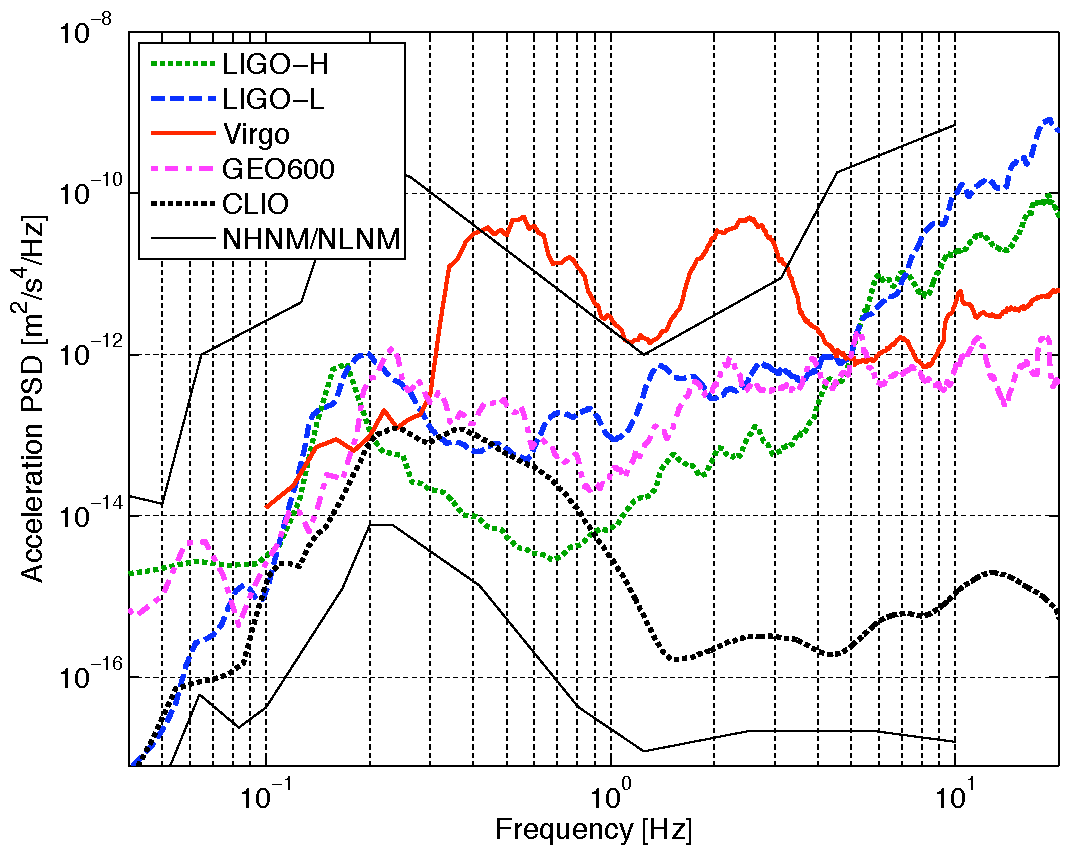
\includegraphics[width=15cm]{./Sec_SiteInfra/Figures/GWD_spectra3.pdf}
		\caption{Seismic acceleration PSD at current gravitational wave detector sites. The magenta dotted line represents the most critical seismic performance limits, which are set by gravity gradient noise.}
		\label{fig3.2}
	\end{center}
\end{figure}

For Einstein Telescope the critical frequencies $f$ are in the range 0.1 - 10 Hz, where the seismic noise is variable mainly due to microseismic and anthropogenic activity. It is therefore important to chose a site location far from oceans and human activities (both at present and in future). The NLNM yields a PSD of $1.38 \times 10^{-17}{\rm m}^2/{\rm s}^4/{\rm Hz}$ at 1 Hz corresponding to an acceleration of $3.7 \times 10^{-9}{\rm m/s}^{2}$. Like the NLNM many remote sites show an approximately flat PSD response for accelerations in the frequency band of 1 - 10 Hz. Corresponding displacements can be found by double integration of the accelerations yielding a $1/\omega^2$ frequency dependence. The conversion should take the integration bandwidth into account (often 1/3 octave is used corresponding to a range of $\pm 10 \%$ about the center value). Note that when a Gaussian signal is passed through a narrow-band filter, the absolute peak signals of the filtered signal envelope will have a Rayleigh distribution (yielding a factor $1.253 \sigma$ for $\vert \overline{x}_P \vert$). Using the above, we find that the lowest possible displacements, according to the NLNM, are about 0.1 nm/$\sqrt{\rm Hz}$ at 1 Hz and decrease with $f^{-2}$.

Presently, the large interferometric detectors GEO600, LIGO, and Virgo are placed on the surface of the earth and, consequently, are sensitive to seismic disturbances. Virgo has already demonstrated good performance above 40Hz, due to a suitable attenuation scheme. Upgrades to LIGO and Virgo will employ further seismic noise reduction by improving their respective active and passive vibration isolation systems. Fig. \ref{fig3.2} shows a comparison of seismic acceleration power spectral densities of the GEO, CLIO (the location for LCGT), Virgo, and LIGO Hanford and Livingston sites. From these ground motion measurements it is clear that the level of seismic noise reduction in the underground environments of CLIO will be less stringent by several orders of magnitude. For Einstein Telescope, the interferometer test masses will be suspended from even more sizeable and complex seismic attenuators, which scheme is discussed in chapter 4. Using these scaled versions of the Virgo super-attenuator at a site that has a low seismic noise background ensures that the ET-D target sensitivity can be reached. 

\begin{figure}[t!]
	\begin{center}
		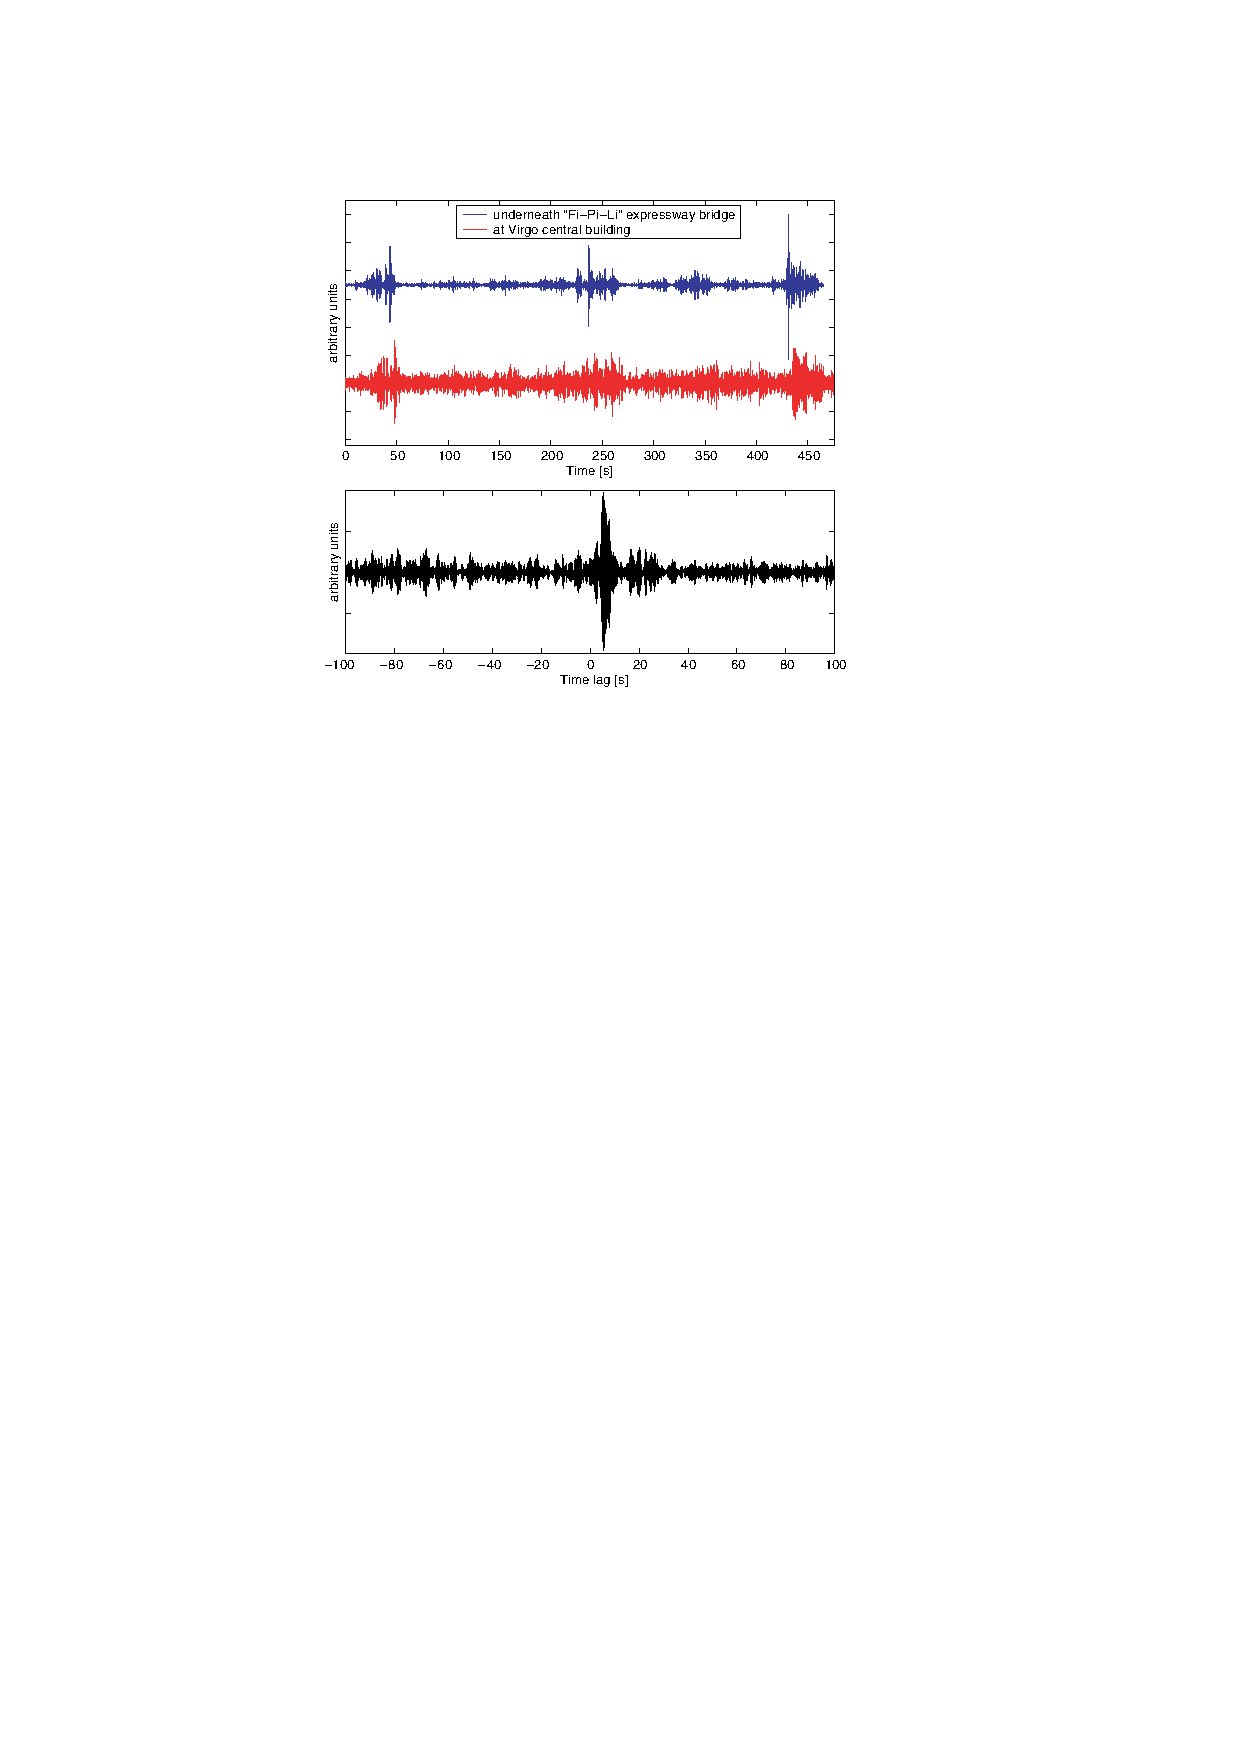
\includegraphics[width=12cm]{./Sec_SiteInfra/Figures/VirgoRoadNoise.pdf}
		\caption{Top: Seismogram recorded on the ground underneath one of the nearby bridges (top signal) and the simultaneous seismogram recorded at Virgo (bottom signal). Three heavy trucks  were crossing at approximately 5, 230, and 420s. Both signals have been bandpass filtered between 1 and 4\,Hz. Bottom: Cross-correlation of the first 100s between the two seismic channels.}
		\label{roadnoise}
	\end{center}
\end{figure}

\FloatBarrier
\subsubsection*{Anthropogenically generated seismic noise}
As was discussed above, the NLNM is a composite of many different stations and instruments with different geology and in various geographic regions. Therefore, it is not possible to duplicate its response at one specific location. It has been observed that lowest noise is obtained in continental sites with sensors placed in hard rock. Sensors with low PSD values are often at borehole and subterranean stations operated at remote sites, far from cultural, oceanic, and meteorologically induced seismic noise. For siting an observatory, this means that the distance to urban areas, highways, railways, and airports, needs be considered. 

The influence of traffic induced seismicity on gravitational wave detectors has been studied by various authors. Road noise depends on road structure and materials, traffic density and vehicle type and speed. Schofield $et$ $al.$ \cite{Schofield2000} reported that local traffic, from passenger vehicles to heavy trucks, induced vibrations at the LIGO Hanford, WA, site. Vibrations were measured for frequencies in the 1 - 50 Hz range, with maxima around 4 - 12 Hz. At the Virgo gravitational wave site, road noise was analysed by using recordings of the seismic field at the Virgo site and correlating these recordings with measurements underneath a major high way overpass, 4\,km away from the Virgo North arm terminal building~\cite{VIR-NOT-FIR-1390-251}. Seismic noise originating from the nearby traffic was found in frequency ranges of 1 - 4\,Hz, peaking at 3\,Hz. The top plot of Fig. \ref{roadnoise} shows the seismic recordings underneath the overpass and at the Virgo end building. The bottom plot of Fig. \ref{roadnoise} shows the cross-correlation between the two signals during the first 100 seconds. Coward $et$ $al.$ \cite{Coward2003} recorded ground vibrations at the AIGO site in Australia for vehicles passing the instrumentation as close as 24 m. Road noise was visible in the 5 - 30 Hz frequency band.
\begin{figure}[t!]
	\begin{center}
		 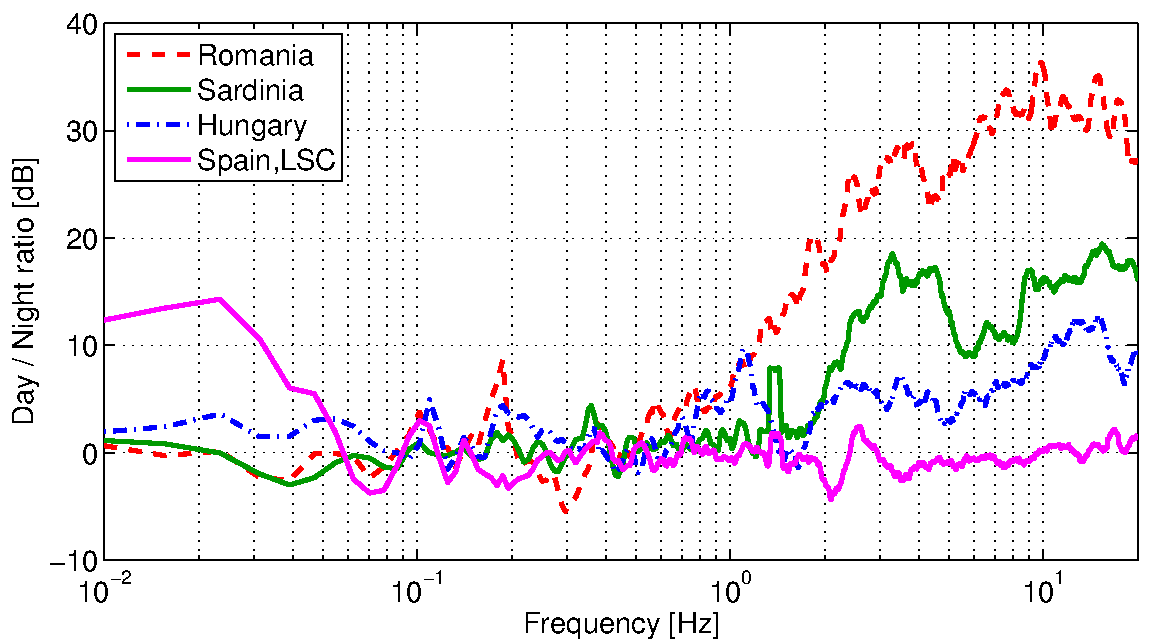
\includegraphics[width=14cm]{./Sec_SiteInfra/Figures/DayNightRatio.pdf}
		\caption{Midday versus midnight noise PSD ratios as a function of frequency at four different measurement sites. Cultural noise is visible for frequencies above 0.7 Hz.}
			\label{fig3.3}
	\end{center}
\end{figure}

Even in remote areas anthropogenic noise can still be recognised. Spectrograms for frequencies up to 60 Hz have been made by Young $et$ $al.$ \cite{Young1996} with seismometers at the surface and within boreholes in the USA for data collected over more than one year. Seismometers were placed in boreholes at Amarillo, TX, at depths of 5, 100, 200, 367, 1219 and 1951 m. The anthropogenic character was present at all depths and exceeded background by about 10 dB. Its source was identified from diurnal patterns and was prominent for frequencies between 1 and 40 Hz. At Datil, NM, seismometers were installed at depths of 0, 5, 43, and 85 m and cultural noise was absent, most probably due to the remoteness of the site. At Pinedale, WY, with seismometers at depths of 3, 13, 30, 122 and 305 m, diurnal patterns in cultural noise were obscured by a pattern of progressive day-time increase of wind noise. 
\begin{table}[h] 
		\centering      % used for centering table
		\caption{Population density at four different measurement sites. Population density figures are given in km$^{-2}$.} 
		\setlength{\tabcolsep}{10pt} 
			\begin{tabular}{l c c c}  % centered columns (4 columns) 
			\hline\hline                        %inserts double horizontal lines 
			Location & Pop. Density & Dist. to ocean/sea & Day/Night @ 10\,Hz \\  % inserts table 
			& [\,km$^{-2}$\,] & [\,km\,] & [\,dB\,] \\ [0.5ex]
			%heading 
			\hline                    % inserts single horizontal line 
			$Romania$ & 180 & 300 & 33  \\   % inserting body of the table 
			$Sardinia$ & 10 & 10 & 16 \\ 
			$Hungary$ & 75 & 500 & 9 \\        % [1ex] adds vertical space 
			$Spain$ & 1.38 & 120& 1 \\ [1ex]       % [1ex] adds vertical space 
			\hline     %inserts single line
			\end{tabular} 
		\label{PopDens}
\end{table} 

As part of the site characterisation, the presence and spectral PSD values of anthropogenic noise were investigated. Fig. \ref{fig3.3} shows an example of the day/night ratio obtained from four different site measurements. Respective high and low frequency disturbances can easily be recognised by comparing the listed day/night ratio values with local population density and the distance to seas and oceans, which are listed in Table \ref{PopDens}. Comparing these statistics, and comparing this with the population density map of Europe in Fig. \ref{fig3.4} (data from REGIO database of Eurostat) collaborates the day/night ratio's found in Table \ref{PopDens}. 
\begin{figure}[t!]
	\begin{center}
		 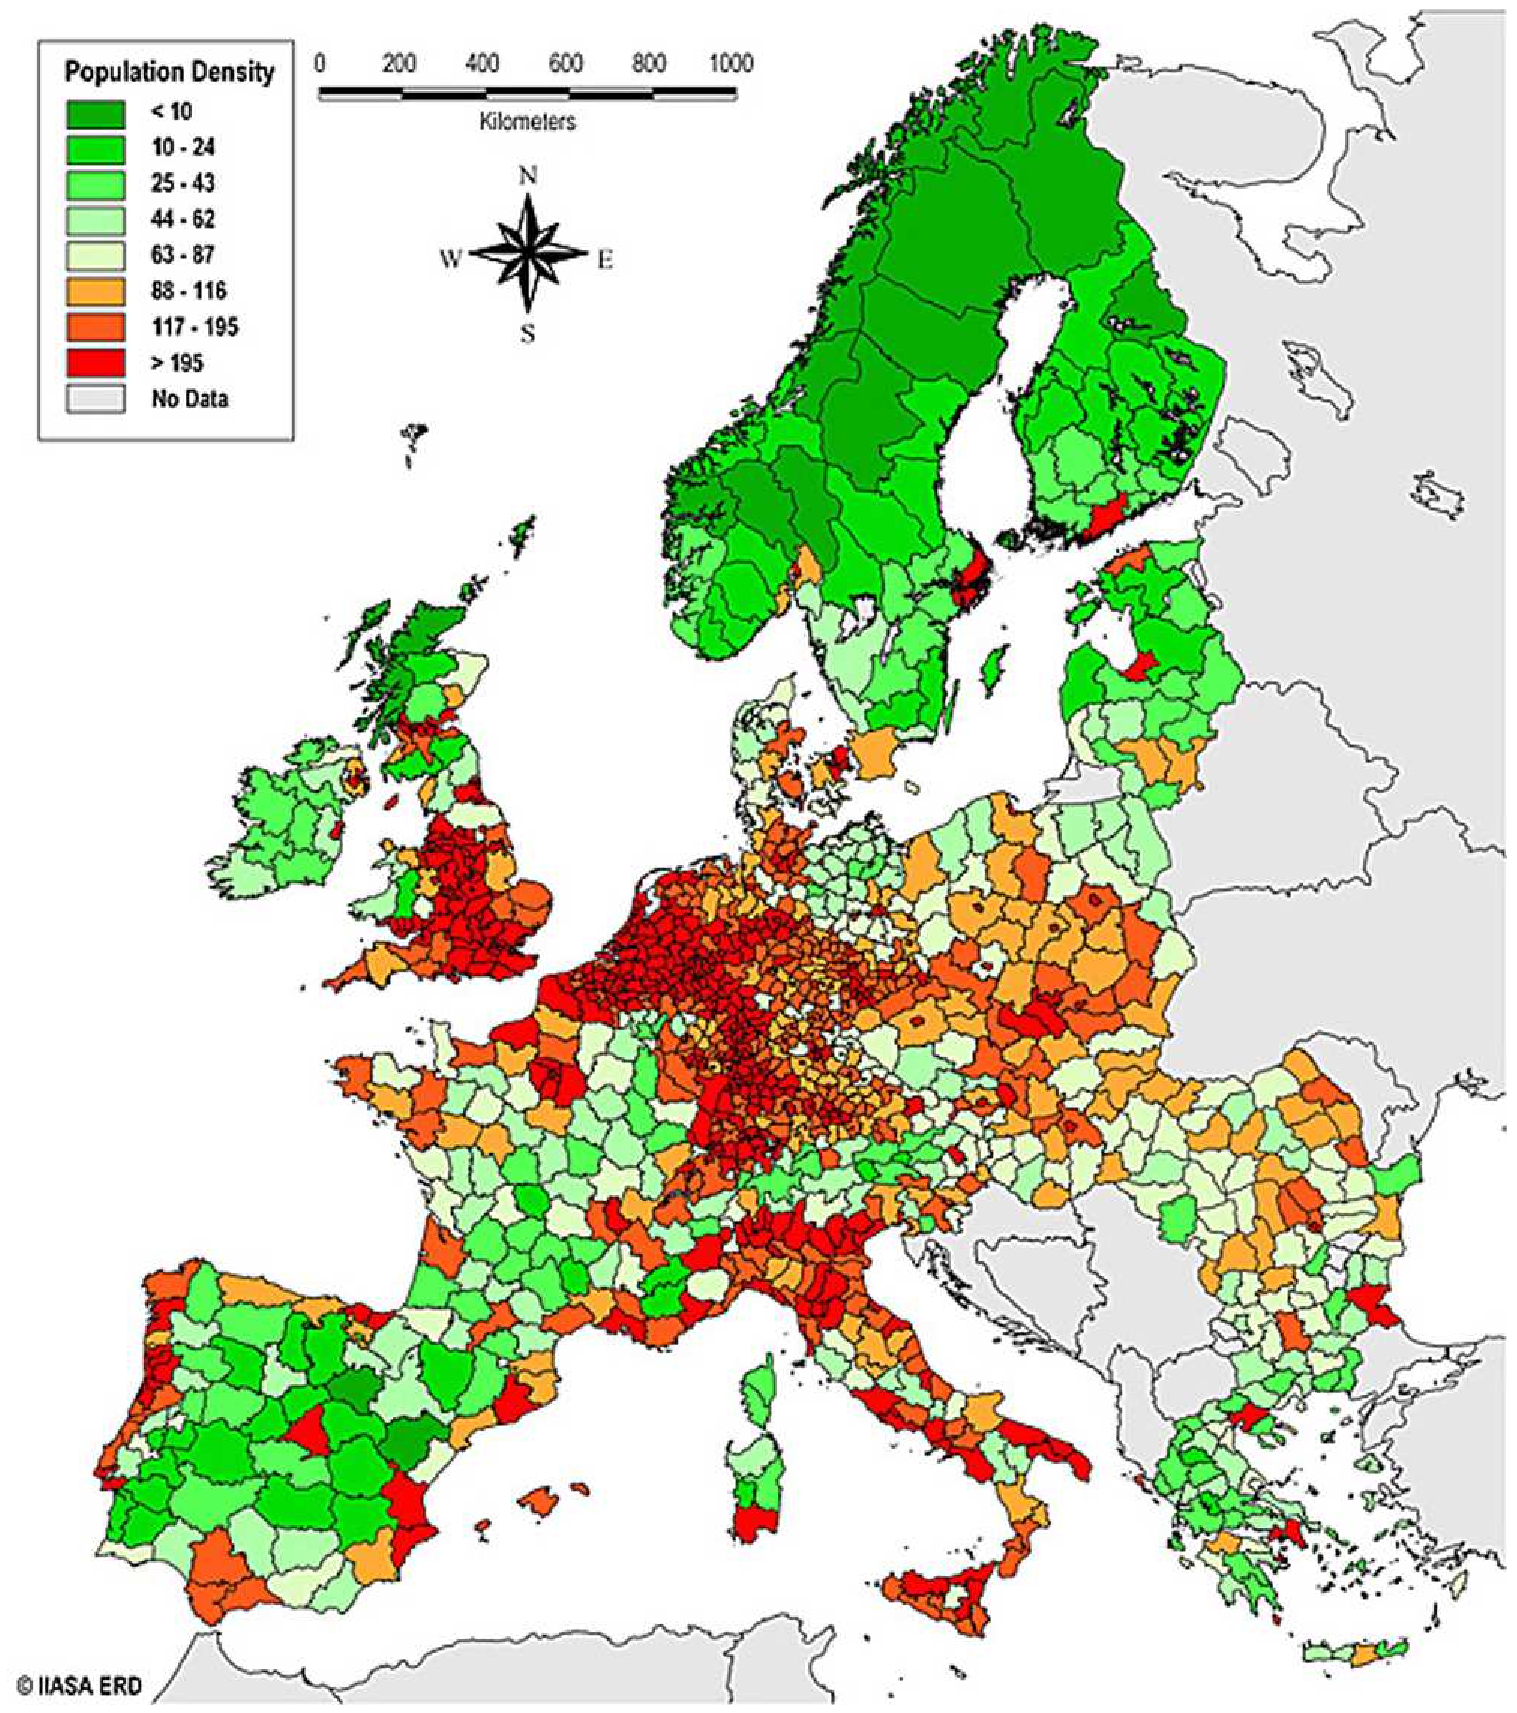
\includegraphics[width=12cm]{./Sec_SiteInfra/Figures/population.pdf}
		\caption{High frequency (1 - 10 Hz) seismic noise is driven by cultural noise. Density of population in Europe from the REGIO database of Eurostat \cite{eurostat}.}
	\label{fig3.4}
	\end{center}
\end{figure}

\FloatBarrier
\subsubsection*{Wind generated seismic noise}
Wind noise has been studied by a number of authors to quantify the conversion of wind energy into ground motion. The presence of wind causes movement of surface objects, such as trees or structures, or directly through turbulent pressures on topographic irregularities. Of particular interest for ET are its frequency range, the wind speed threshold for it to become evident, and its persistence with depth. 

Withers $et$ $al.$ \cite{Withers1996} performed measurements at Datil, New Mexico in the frequency band of 1 - 60Hz. This is a remote site that features sparse vegetation and distances to the nearest road and railroad were 12 and 90 km respectively. Measurements were performed at a depth of 0, 5, 43 and 85 m and the effect of wind noise was evident over the entire observed bandwidth with an ambient background threshold of $\sim$3 m/s. At a depth of 43 m a reduction of 20 dB was found. Slightly higher reduction factors were found at 85 m.
\begin{figure}[h!]
	\begin{center}
		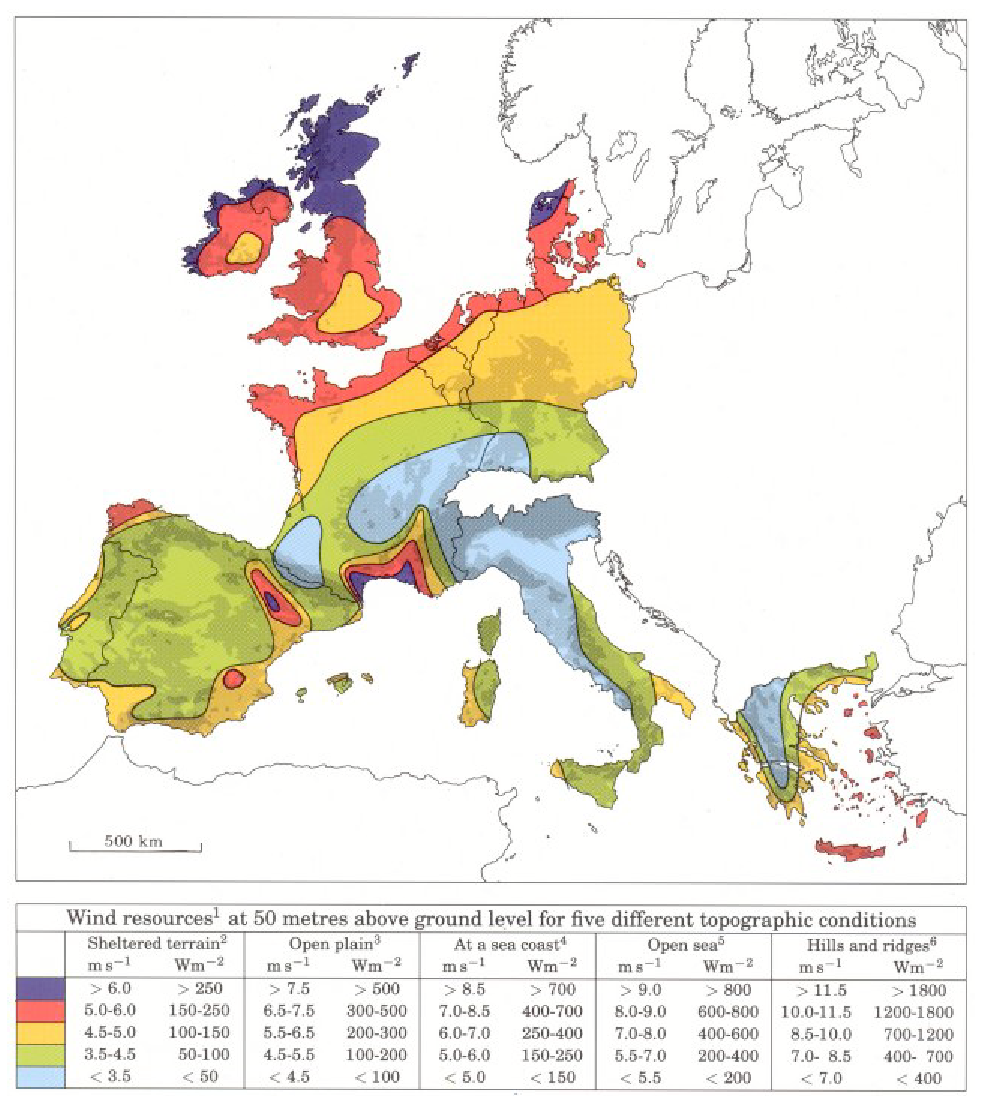
\includegraphics[width=12cm]{./Sec_SiteInfra/Figures/wind.pdf}
		\caption{European wind resources based on data collected for the European Wind Atlas \cite{WindatlasWWW}.}
		\label{fig3.5}
	\end{center}
\end{figure}

Young $et$ $al.$ \cite{Young1996} carried out similar measurements. Wind speed thresholds, for the presence of wind induced background noise, were found to be 3-4 m/s at depths of 0-5 m and 8-9 m/s at depths below 100 m. A strong correlation between seismic noise and wind was observed over a broad frequency spectrum range from 1 to 60 Hz. The noise was 34 dB above the NLNM at a depth of 3 m, and decreased to 10 dB above NLNM at a depth of 305 m. Koller $et al$. (2004) determined that many parameters relating to measured ground motion caused the amplitude ratio to vary, but that only wind speed affected the frequency at which the horizontal to vertical ratio curves peaked. Mucciarelli $et al$. (2005) found that, provided the sensor was sheltered from direct wind (inside a concrete box at 1.5 m depth), wind increased the amplitude of all components of seismic noise (vertical, east-west, north-south) in the band 0.1 - 10 Hz similarly, such that ratio was unchanged. This conclusion was valid for wind speeds up to 8 m/s. 

The reductions in wind noise are a prime example that surface seismic noise contributions will decay with depth. For ET, the underground environment is expected to improve on all sources of seismic noise since surface seismic noise is exponentially reduced with depth, $e^{-4d /\lambda}$, where d is the depth and $\lambda$ is the wavelength of the seismic wave. Fig. \ref{fig3.6} shows results from measurements at the Gy\"ongy\"osorozi mine by Beker $et$. $al$. in the Hungary. A factor of $\sim$10 suppression at 10\,Hz at the depth of 400\,m, and substantially more at higher frequencies. At Gy\"ongy\"osoroszi, the speed of sound at 400\,m underground (hardrock) is about 3\,km/s, implying that the seismic waves in the 0.1 - 10\,Hz band have long wavelengths that at the surface: 300\,m - 30\,km.
\begin{figure}[h!]
	\begin{center}
		 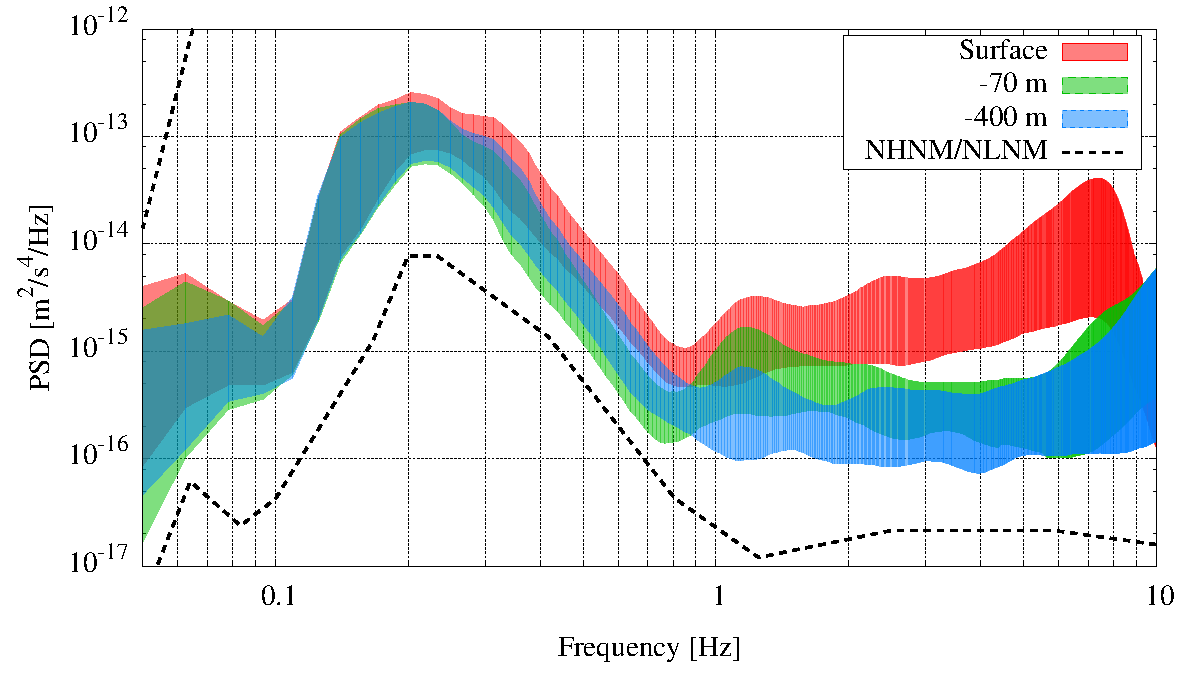
\includegraphics[width=15cm]{./Sec_SiteInfra/Figures/Hung_transparent2.pdf}
		\caption{Measured reduction of seismic noise at the Gy\"ongy\"osorozi mine in Hungary for three different seismic sensors at depths of 0, 70, and 400 m.}
		\label{fig3.6}
	\end{center}
\end{figure}

\FloatBarrier
\subsubsection{Geological and geographic observations}
McNamara and Buland \cite{mcnamarab} have carried out a study of geographic dependence of ambient seismic noise in the USA. Fig. \ref{OneGeologyPic} shows that the strongest geographic dependence is obtained for frequencies above 1 Hz (panel A). Noise levels at the East coast are up to 50 dB above NLNM due to large population centers and represents cultural noise. Microseism shows up in the 0.125 - 0.25 Hz frequency range (panel B) and is dominant is coastal regions. The US continental interior has noise levels about 10 dB above NLNM.
\begin{figure}[h!]
	\begin{center}
		 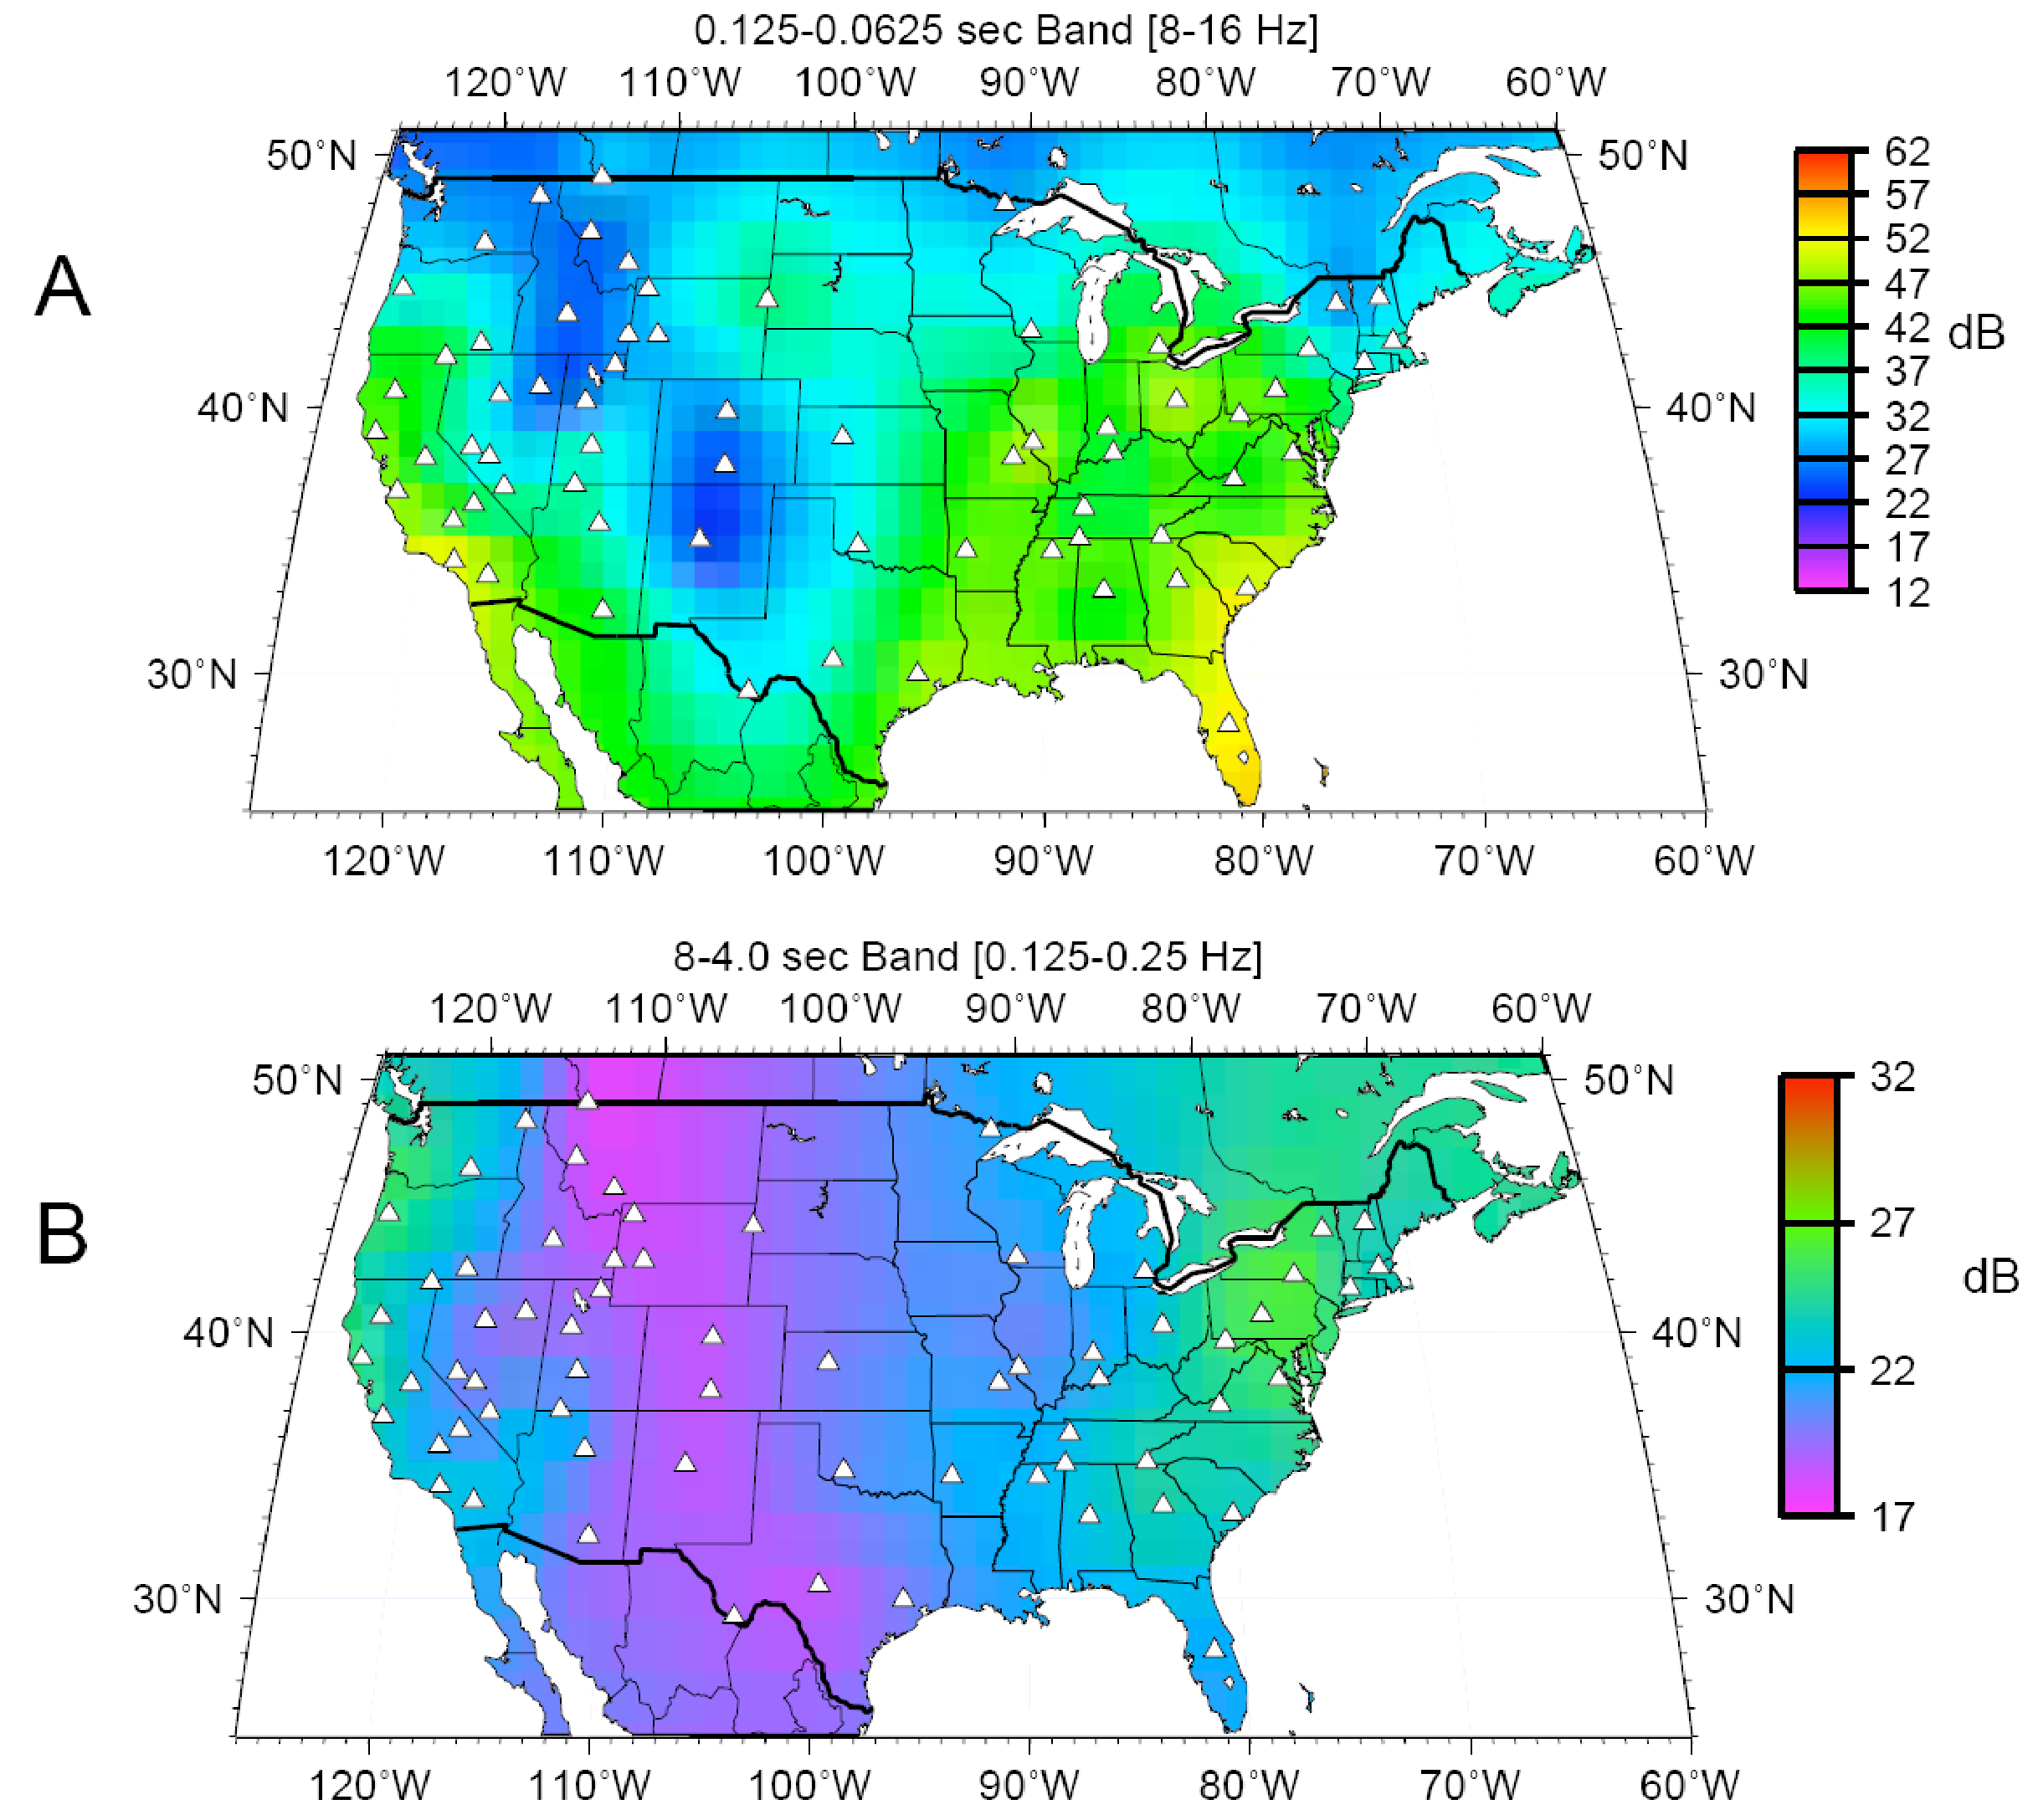
\includegraphics[width=15cm]{./Sec_SiteInfra/Figures/Geo.pdf}
		\caption{PSD noise levels above the NLNM mapped across the US in two separate frequency bands \cite{mcnamarab}: panel A or 8 - 16 Hz and panel B for 0.125 - 0.25 Hz.}
		\label{OneGeologyPic}
	\end{center}
\end{figure}


\noindent
Recently, OneGeology \cite{onegeology}, an ambitious online project, under the direction of the British Geological Survey, started the collection of worldwide geological information. Large areas of alluvium can be identified in Europe. Allivium is deposited soft soil composed of silt, clay, sand and gravel. Its material properties vastly differ from hard rock such as granite. This has immediate consequences for the ambient seismic noise levels. The seismic data have been obtained with the ORFEUS (Observatories and Research Facilities for European Seismology) network, a non-profit foundation that aims at co-ordinating and promoting digital, broadband seismology in the European-Mediterranean area. For frequencies around 2 Hz the seismic noise is almost 40 dB higher in alluvium (stationa GE.HLG) than hardrock (station CH.GIMEL). This is caused by the lower velocity of seismic waves in sediments compared to hardrock. Areas dominated by alluvium can be found in the Netherlands, northern Germany and Poland, in the south of Germany, northern Italy (Po area), Toleda area in Spain, and eastern Europe. PSD values about 40 dB larger than hardrock have also been found in alluvium regions near Bejing, China and Santa Barbara, USA. Although for a surface site such regions should be avoided, this is not at all clear for an underground site.



\noindent
Results of a systematic investigation of ambient noise in Germany \cite{steinwachs} were made by Steinwachs. Noise levels are lowest for sites in the south of Germany where geology is determined by kristalline granite formations. Highest ambient noise levels are recorded in the north of Germany where the hardrock layers are covered by alluvium (molasse). In between layers of harder Jura formations cover the crystalline granite. Average spectral densities are fitted with exponential functions because of strong oscillations in PSD values. The signal at 2 Hz for the smallest spectral densities has been traced by a directional analysis to Rayleigh waves originating from the coast of Norway. The signal is believed to be due to choppy water waves in the shallow North Sea hitting the shore.

\noindent
At first sight it may be thought that Scandinavia may provide suitable sites, since it is scarcely populated leading to low cultural noise, while the surface is dominated by old, good crystalline hardrock. However, seismic measurements from the KONO station near Kongsberg, Norway, show PSD values 20 - 30 dB above the NLNM (typically -140 dB around 1 Hz). It should be noted that the KONO sensor is located in a silver mine at 340 m depth. The ambient seismic noise is due to the high frequency tail from the microseismic peak. KONO data show that the microseismic peak show large seasonal variations. Moreover, in the winter months seismic noise can be expected from ice activities in the Baltic Sea.

